%%~~~~~~~~~~~~~~~~~~~~~~~~~~~~~~~~~~~~~~~~~~~~~~~~~~~
\frame{
\frametitle{GUI: Programmaufbau}
	\begin{block}{Anforderungen}
		\begin{itemize}
			\item Basisklasse GUI enth�lt m�gliche Designelemente f�r einzelne Abschnitte der APP
			\item Seiten erben von Basisklasse und implementieren eigene Funktionalit�t
		\end{itemize}
	\end{block}
}

\frame{
\frametitle{Gui: Klassendiagramm}
	\begin{center}
			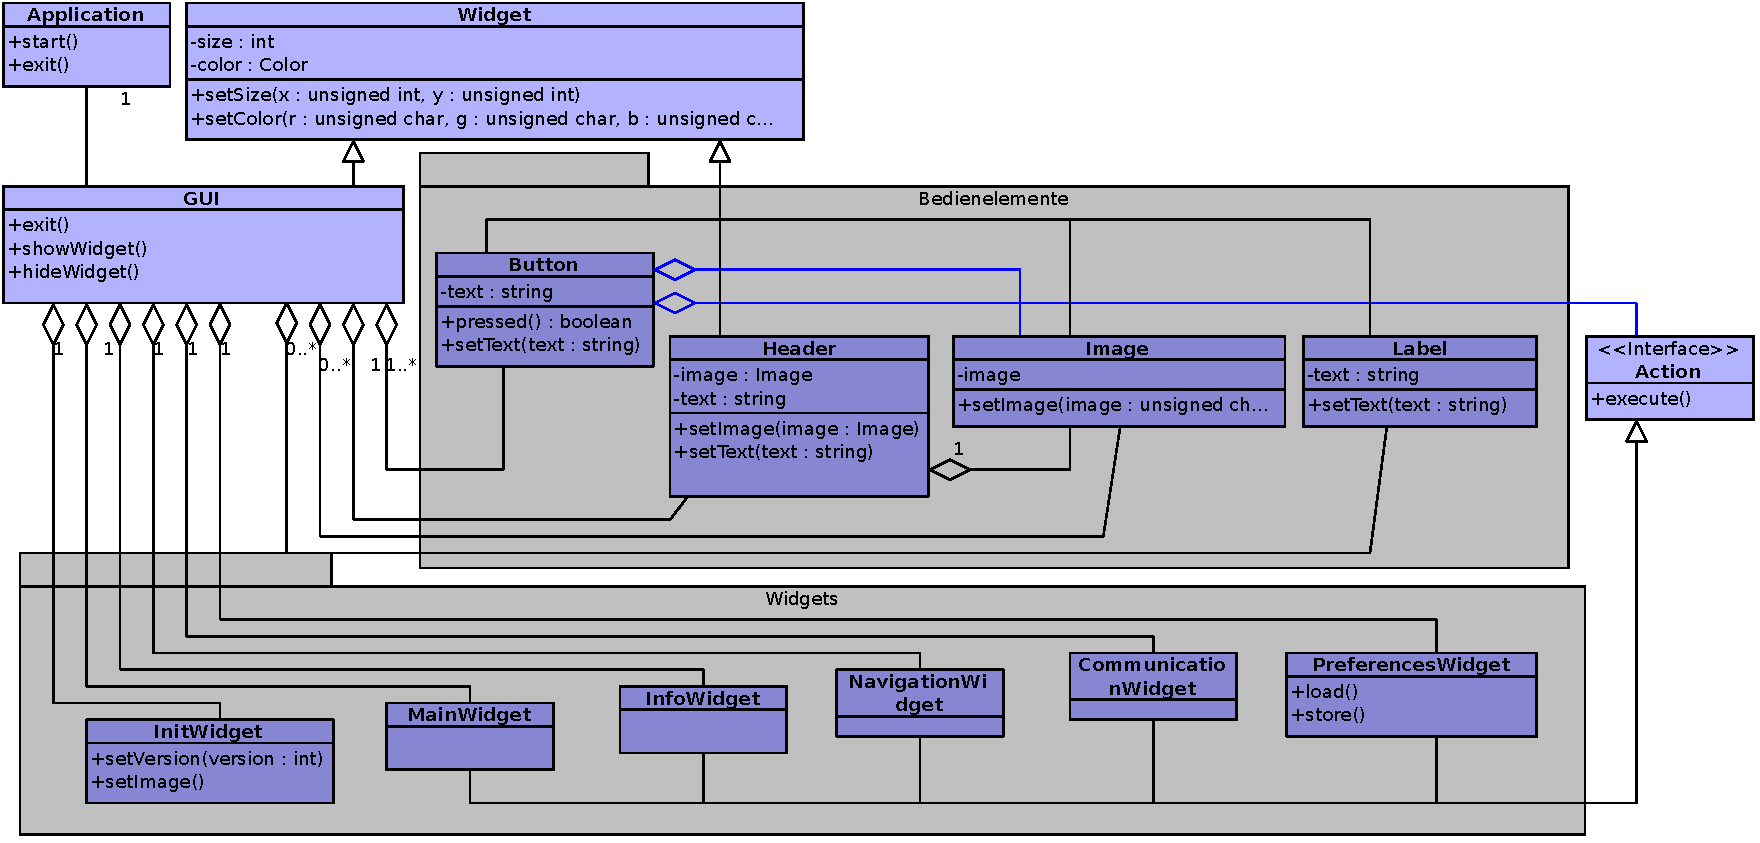
\includegraphics[width=0.9\textwidth]{../grafiken/GUI_Class.pdf}
	\end{center}
}


\frame{
\frametitle{Men�wechsel}
	\begin{block}{Zustandsmaschine}
		\begin{itemize}
			\item Men�punkte werden als Zustand gesehen
			\item zus�tzliche Zust�nde f�r Start und Beenden der Application
			\item Zust�nde k�nnen wiederum Unter-Zust�nde besitzen
		\end{itemize}
		\begin{center}
			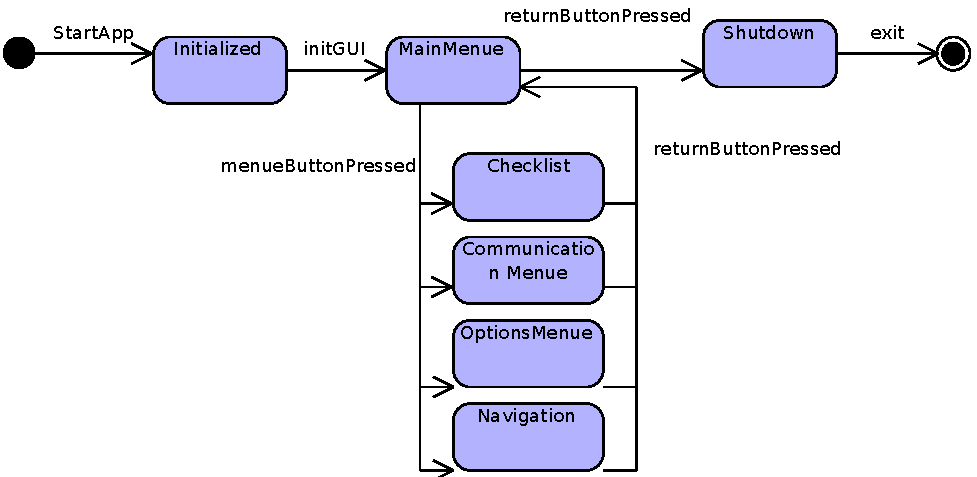
\includegraphics[width=0.65\textwidth]{../grafiken/MenueStates.pdf}
		\end{center}
	\end{block}
}